\documentclass[12pt,a4paper]{article}
\usepackage{float}
\RequirePackage[T1]{fontenc}
\RequirePackage[english]{babel}
\RequirePackage[dvips]{graphicx}
%\RequirePackage[textures]{color}
\RequirePackage[dvips]{color}
\usepackage{amsmath}
\usepackage{alltt}
\usepackage{verbatim}
\usepackage{float}

\definecolor{SifCol}{rgb}{0.5,0.5,0.5}
\newcommand{\sifitem}[2]{\item[\tt{#1}]\hspace{1mm}{\color{SifCol}\hspace{1mm}\tt{#2}}\newline} 

\newcommand{\sifbegin}{\begin{description}}
\newcommand{\sifend}{\end{description}}

\newcommand{\Der}[2]{\frac{\partial{#1}}{\partial{#2}}}
\newcommand{\Inv}[1] {\frac{1}{#1}}
\newcommand{\ttbegin}{\begin{alltt}}
\newcommand{\ttend}{\end{alltt}}
\newcommand{\keno}{$\backslash$}

\newcommand{\code}[1]{\texttt{#1}}

\floatstyle{ruled}
\newfloat{listing}{tp}{.lst}
\floatname{listing}{Listing}


\begin{document}
\title{ElmerParam Manual}
\author{Erik Edelmann and Peter R�back}
\date{\today}
\maketitle
%\tableofcontents

\section{Introduction}

ElmerParam is a simple tool for parametrized computation for software
that uses ASCII-format input and output files. It was primarily designed to
be used with Elmer, but can easily be used with other software packages as
well.  The parametrized approach is particularly useful for optimization
purposes.

ElmerParam exists both as a standalone program and as a library with
bindings for C, Fortran, R and Matlab.

In this document, the following designations are used:
\begin{tabbing}
    \code{[whatever]} \hspace{2em} \= \code{whatever} is optional.\\
    $A$|$B$              \> either $A$ xor $B$.\\
    %\textit{<numexpr>}   \> \parbox[t]{0.70\textwidth}{can be either a
    %                        literal numerical constant or a ``\code{\$}''
    %                        followed by a MATC expression.  See section
    %                        \ref{MATC} for more on MATC}\\
    \code{\$\{ELMER\_HOME\}} \> \parbox[t]{0.70\textwidth}{Environment
                            variable supposed to be set to the directory
                            where Elmer (including ElmerParam) was
                            installed.}\\
    ElmerParam  \> (in normal font) The ElmerParam package.\\
    \code{ElmerParam} \>  (\code{this font}) The standalone
                          \texttt{ElmerParam} program.

\end{tabbing}


\section{General overview}

\begin{figure}
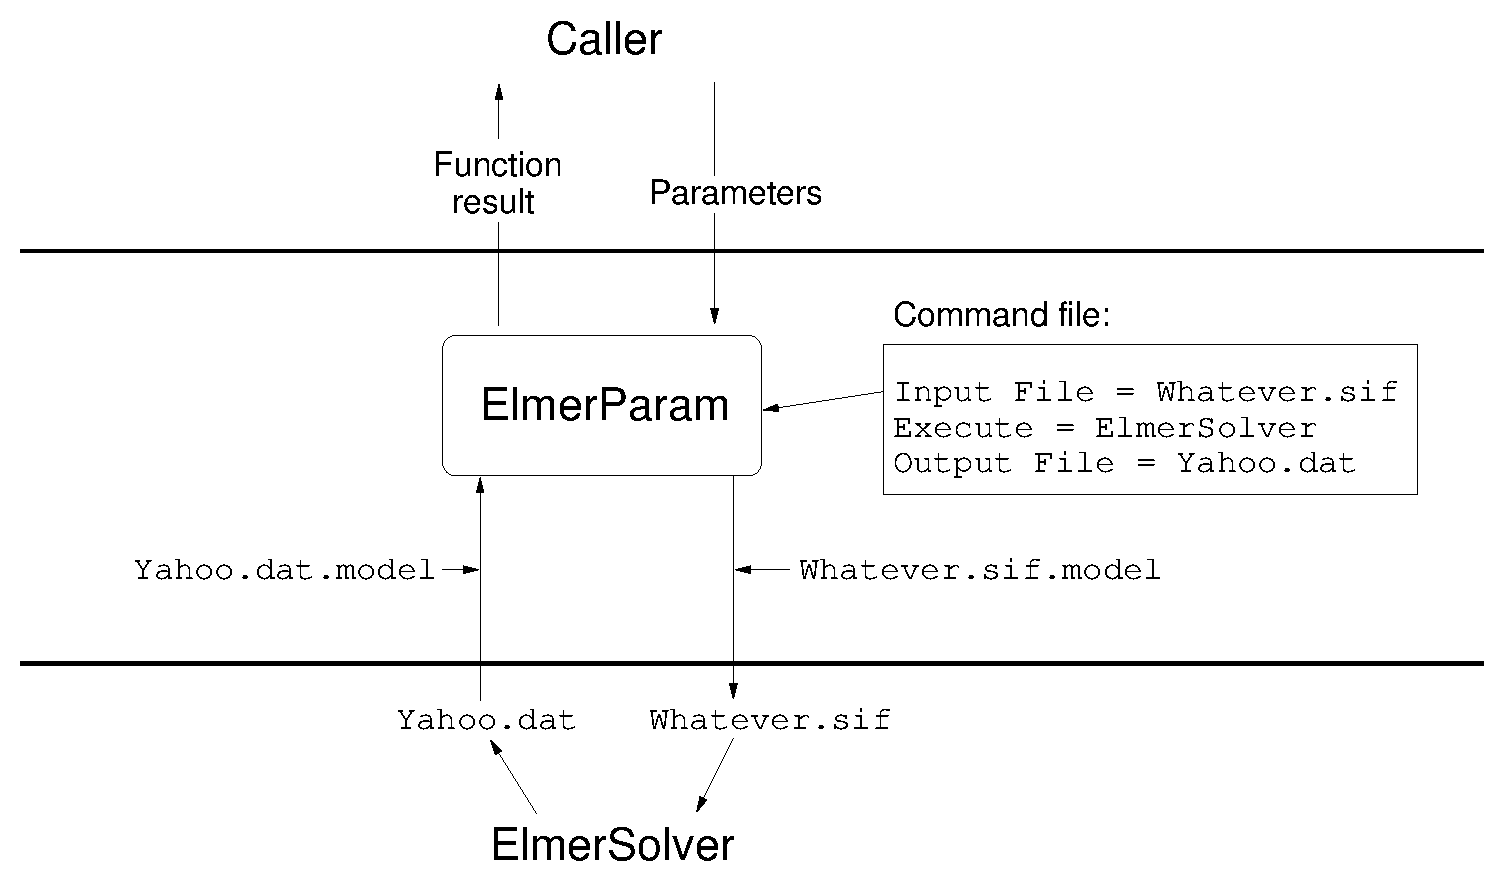
\includegraphics[width=\textwidth]{ep.eps}
\caption{ElmerParam as a layer between ElmerSolver and a program that
wants to call ElmerSolver as function of some parameters.}
\end{figure}

ElmerParam acts a layer between computational programs such as ElmerSolver
and programs that wants to call the computational programs as functions of
some parameters.  It provides functions which take real and/or integer
parameters as arguments, and return a scalar or vector of real output
values:
\begin{align*}
    f:& \mathbf{R}^n \times \mathbf{Z}^m \longrightarrow \mathbf{R}
    \intertext{or}
    f:& \mathbf{R}^n \times \mathbf{Z}^m \longrightarrow \mathbf{R}^k
\end{align*}
where $n$ is the number of real parameters, $m$ the number of integer
parameters, and $k$ the length of the return vector.  These functions are
from the caller's point of view black boxes and therefore no information
about the case is provided. This information is instead provided in a set
of files read by ElmerParam.

The most important file is a ElmerParam command file, which
contains the commands to run the computation programs. A typical command file
will create input files with parameter values for the computation program,
execute the computation program, and read parameter values from it's output
files.  The input files are created and output files interpreted with the
help of template (model) files. Simple calculations specified in the MATC
language can be performed by ElmerParam itself (see section \ref{MATC}).

In addition to computation parameters, ElmerParam can also be given a
special ``tag'' parameter. The tag can be expanded not only in the input
files, but also be used in the command file.  It can be used to give unique
names to all the input and output files, which can be important when
running several instances of ElmerParam in parallel.

\section{ElmerParam Files}

ElmerParam routines need a number of different files with information on
the problem to be solved.

\begin{itemize}
\item The \texttt{ELMERPARAM\_STARTINFO} file has a fixed 
	name and has only one line, the name of the ElmerParam command file.
\item ElmerParam command file is the file containing the execution instructions 
	needed for the evaluation of the function return value. 
\item Each case needs a set of model files that are generalized versions of
    the input and output files.  In the model files the parameters are
    given in brackets.  For example the first real valued parameter is
    inserted where \code{<!R1!>} occurs.  Input file models are used to create
    input files for the computation of, for example, ElmerGrid or
    ElmerSolver.  Output file models are used to read result information
    from the output file. 
\end{itemize}


\subsection{ElmerParam command file}

The ElmerParam command file includes some simple statements that are run in
the order of appearance. The general form of a statement is
\ttbegin
Command = argument
\ttend
Commands are case insensitive. Lines starting with \code{\#}, \code{!} or
\code{*} are ignored. A statement can be split onto several lines by
putting a '\keno' as the last character on a line.  \code{<!T!>} in an
argument will be expanded to the value of the tag parameter.


\subsubsection{Commands:}
\begin{description}

\item{\code{Comment = string}}

Echo \code{string} to stdout.

\item{\code{Echo = True|False}}

Turn ECHO on|off.  If `on', all commands are echoed to stdout when executed.
`On' by default.

\item{\code{Matc = True|False}}

Turn MATC support on|off. Has to be `on' if you use MATC expressions.
Requires that ElmerParam was compiled with MATC support. Off by default.  

\item{\code{Input File = fname1 [Using fname2]}}

Create the file \code{fname1} from the model file
\code{fname2}. If no model file name is given, the name
\code{fname1.model} is assumed.

\item{\code{Execute = cmd}}

Execute the shell command \code{cmd}.  Usually this would be the
computation part, or mesh generation if using parametrized mesh
generation.

\item{\code{Output Files = fname1 [Using fname2]}}

Read parameters from the output file \code{fname1} using the model file
\code{fname2}. If \code{fname2} isn't given, \code{fname1.model} is
assumed.

\item{\code{Save File = fname}}

Save history data of all the computations in file \code{fname}.  If
this keyword is active all the input parameters and the function return
value are saved to a line that is appended in the given file.

%\item{\code{Parameter X$n$ = }\textit{<numexpr>}}
%
%Assign a value to parameter \code{X$n$}, where \code{X} is either \code{I}
%for integer parameter, or \code{R} for real.

%\item{\code{Parameter min|max X$n$ =} \textit{<numexpr>}}
%
%Set a minimum|maximum value for parameter X$n$. If the parameter lies
%outside the defined limits then the routine is terminated and a default
%value for the function is returned.

%\item{\code{[Cost] Function  =} \textit{<numexpr>}}
%
%Set the return value (scalars only).  Note that the return value can also
%be read from an output file as the special parameter O.

\item{\code{\$}\textit{<expression>}}

Use MATC to evaluate the MATC expression \textit{<expression>}.  See
section \ref{MATC} for more.

\end{description}

Below is a simple example of a ElmerParam command file. 
\ttbegin
#
# This comment will be ignored.
#
Comment = ElmerOptim routine 
Echo = True
Input File = OptimTemp2.sif
Execute = ElmerSolver
Output File = cost.dat
Save File = evals.dat
\ttend

\subsubsection{MATC extension}\label{MATC}

The ElmerParam includes the MATC language written by Juha Ruokolainen that
may be used, for example, to evaluate the values of the parameters.  The
MATC extensions are by default not evaluated and the variable \code{MATC}
need to be set \code{True} to activate the library. 

In MATC, the real parameters are stored in a vector called \code{R}, 
integer paremeters in the vector \code{I}, and the function result in the
vector \code{O}.  Thus, \code{R}$n$ can be
accessed through \code{R($n$)}, and so on.

Below is an example command file that shows how the MATC library may be
used.
\ttbegin
Comment = Testing routine
MATC = True
\$ apu1 = R(0) + R(1)
\$ apu2 = sin(apu1)
\$ R(1) = apu2 
\$ I(0) = 5
\$ I(1) = sum(I(2:4))
\$ O = R(0) + R(1) + I(0)
\ttend



\subsection{Model files}\label{modelfiles}

\subsubsection{Creating Input files}
When creating an input file, ElmerParam simple copies the contents
of the model file, expanding parameter references where they occur.
A parameter reference in the model file has the form
\ttbegin
<!ParamSpec[\verb+^+]!>
\ttend
where \code{ParamSpec} can be:
\begin{table}[H]
\begin{tabular}{ll}
T           & The tag parameter\\
X$n$        & Parameter of type 'X' and index $n$.\\
X($n$:$m$)  & A vector of parameters from X$n$ to X$m$.\\
X           & A vector of all parameters of type 'X'\\
\end{tabular}
\end{table}
\noindent Here `X' can be `R' for real, or `I' for integer.  Note that
indexing starts at 0; thus the first real parameter will be R0, the second
R1, and so on.  An optional transpose operator \verb+^+ after the
\code{ParamSpec} denotes that it is a column vector (vectors are by default
row vectors.).  If a line contains a column vector, it will be repeated $n$
times, where $n$ is the lentgh of the vector, with the $i$:th vector
component at the $i$:th copy of the line.  If a line contains more than one
columns, they have better be of the same length, or the vicious Yeti will
eat your computer.

Example: if the model file looks like
\begin{verbatim}
r = <!R0!>
i = <!I!>
  Temperature = Variable Coordinate 2
    Real
        <!R(1:19)^!>     <!R(20:38)^!>
    End
\end{verbatim}
and I = [ 1, 2, 3 ], R0 = 1.0, R(1:19) = [ 0.0, 0.2, 0.4 \ldots{} ], and
R(20:38) = [ 1.0, 2.0, 3.0, \ldots{} ] the input file becomes
\begin{verbatim}
r = 1.0
i = 1  2  3
  Temperature = Variable Coordinate 2
    Real
        0.0     1.0
        0.2     2.0
        0.4     3.0
         .       .
         .       .
         .       .
    End
\end{verbatim}


\subsubsection{Reading Output files}
When reading parameter values from an output file using a model file,
ElmerParam will skip everything in the output file except those places
where there is a parameter reference in the model file, in which case
ElmerParam reads values from these places in the output file into the
specified parameters.

The parameter references for output files has the same general form as for
input files, where \code{ParamSpec} in this case can be
\begin{table}[H]
\begin{tabular}{ll}
X$n$        & The $n$:th parameter of type 'X'.\\
X($n$:$m$)  & A vector of parameters from X$n$ to X$m$.\\
X           & A vector of all parameters of type 'X'\\
\end{tabular}
\end{table}
\noindent where `X' can be `R' for real, `I' for integer, or 'O' (uppercase
'o') for function result.

For example, if the model file looks like
\begin{verbatim}
r = <!R!>
i = <!I0!>
y = <!O(0:4)^!> <!O(5:9)^!>
\end{verbatim}
and the output file is
\begin{verbatim}
r = 1.0 2.0 3.0
i = 6
y = 1.0     6.0
    2.0     7.0
    3.0     8.0
    4.0     9.0
    5.0    10.0
\end{verbatim}
ElmerParam will read [ 1.0, 2.0, 3.0 ] into R(0:2)
(assuming the number of real parameters is 3), 6 into I0, and
[ 1.0, 2.0, 3.0, 4.0, 5.0, 6.0, 7.0, 8.0, 9.0, 10.0 ] into O(0:9).

\section{Interfaces}

\subsection{Standalone program}

\begin{verbatim}
ElmerParam [inputfile [outputfile [tag]]]
\end{verbatim}
\begin{description}
\item{\tt inputfile:} Name of file containing input parameters (use '-' or
leave empty for
stdin).  It shall have the following format:
\begin{verbatim}
[nr
R0
R1
.
.
.
[ni
I0
I1
.
.
.
[nfun]]]
\end{verbatim}
If \texttt{nfun} is absent, 1 will be assumed.  Example:  Three real
parameters, no integer parameters, and 3 output parameters:
\begin{verbatim}
3
1.0
2.0
3.0
0
3
\end{verbatim}
\item{\tt outputfile:} Name of file where output parameters will be written
in a column (use '-' or leave empty for stdout).
\item{\tt tag:} Optional tag parameter.
\end{description}


\subsection{C interface}

\begin{verbatim}
#include <elmerparam.h>

double elmer_param(int nr, const double *xr, int ni, const int *xi,
                   const char *tag)

void elmer_param_vec(int nfun, double *fun,
                     int nr, const double *xr, int ni, const int *xi,
                     const char *tag)
\end{verbatim}
\begin{table}[H]
\begin{tabular}{ll}
    \code{nfun} &Number of output parameters. (\code{elmer\_param\_vec}
    only)\\

    \code{fun} &\parbox[t]{10cm}{Array of output parameters, corresponds to
    O(0:\code{nfun}-1) in the ElmerParam input files.  Must be big enough to
    hold \code{nfun} values. (\code{elmer\_param\_vec} only.)}\\

    \code{nr} &Number of real parameters.\\

    \code{xr} &\parbox[t]{10cm}{Array of real parameters, corresponds to
    R(0:\code{nr}-1) in the ElmerParam input files. (Use \code{NULL} for no
    real parameters.)}\\

    \code{ni} &Number of integer valued parameters.\\

    \code{xi} &\parbox[t]{10cm}{Array of integer parameters, corresponds to
    I(0:\code{ni}-1) in the ElmerParam input files.  (Use \code{NULL} for no
    integer parameters.)}\\

    \code{tag} &Tag parameter. (Use \code{NULL} for no tag.)\\

    Return value &\parbox[t]{10cm}{Scalar output parameter, corresponds to
    O (or O0) in the ElmerParam input files. (\code{elmer\_param} only.)}

\end{tabular}
\end{table}

\noindent To compile a C code that calls \code{elmer\_param()}, add
\ttbegin
-I\$\{ELMER\_HOME\}/include
\ttend
to the compiler flags.  For linking, add
\ttbegin
-L\$\{ELMER\_HOME\}/lib -lelmerparam -lmatc -lm
\ttend
to the linker flags. (\code{-lmatc} can be omitted if ElmerParam was
compiled without MATC support).


\subsection{Fortran interface}

\begin{verbatim}
use elmerparam

interface elmer_param

    function elmer_param_scal (xr, xi, tag) result(y)
        double precision, optional, intent(in) :: xr(:)
        integer, optional, intent(in) :: xi(:)
        character(*), optional, intent(in) :: tag

        double precision :: y
    end function elmer_param_scal

    function elmer_param_vec (nfun, xr, xi, tag) result(y)
        integer, intent(in) :: nfun
        double precision, optional, intent(in) :: xr(:)
        integer, optional, intent(in) :: xi(:)
        character(*), optional, intent(in) :: tag

        double precision :: y(nfun)
    end function elmer_param_vec

end interface elmer_param
\end{verbatim}
\begin{table}[H]
\begin{tabular}{ll}
    \code{nfun} &Length of return vector (\code{elmer\_param\_vec} only).\\

    \code{xr} &\parbox[t]{10cm}{Array of real parameters, corresponds to
    R(0:\code{size(xr)}-1) in the ElmerParam input files.}\\

    \code{xi} &\parbox[t]{10cm}{Array of integer parameters, corresponds to
    I(0:\code{size(xi)}-1) in the ElmerParam input files.}\\

    \code{tag} &Tag parameter.\\

    Return value &\parbox[t]{10cm}{
    \code{elmer\_param\_scal}: Scalar output parameter, corresponds to O (or O0)
    in the ElmerParam input files.
    
    \vspace{1ex}

    \code{elmer\_param\_vec}: \code{nfun} Output parameters, corresponds to
    O(1:\code{nfun}) in the ElmerParam input files.}\\

\end{tabular}
\end{table}

\noindent To compile a Fortran code that USEs \code{elmerparam}, add
\ttbegin
-I\$\{ELMER\_HOME\}/include
\ttend
to the compiler flags. You'll have to replace ''\code{-I}'' with whatever
option your compiler uses to tell where to look for \code{*.mod} files.
This varies from one compiler to another -- check the documentation of your
compiler\footnote{Most compilers uses \code{-I}; among the exceptions are
Sun f95 which uses -M.}.  Also note that you have to use the same compiler
that was used to compile ElmerParam.  For linking, add 
\ttbegin
-L\$\{ELMER\_HOME\}/lib -lelmerparamf -lelmerparam -lmatc -lm
\ttend
to the linker flags. (\code{-lmatc} can be omitted if ElmerParam was
compiled without MATC support).


\subsection{R interface}

\begin{verbatim}
library("elmerparam")

elmer_param <- function(xr = NULL, xt = NULL, xi = NULL, tag = "", nfun = 1)
\end{verbatim}
\begin{table}[H]
\begin{tabular}{ll}
    \code{xr} &\parbox[t]{10cm}{Array of real parameters, corresponds to
    R(0:\code{length(xr)}-1) in the ElmerParam input files.}\\

    \code{xi} &\parbox[t]{10cm}{Array of integer parameters, corresponds to
    I(0:\code{length(xi)}-1) in the ElmerParam input files.}\\

    \code{tag} &Tag parameter.\\

    \code{nfun} &Length of return vector.\\

    Return value &\parbox[t]{10cm}{
    Vector of output parameters, corresponds to
    O(0:\code{nfun}-1) in the ElmerParam input files.}\\

\end{tabular}
\end{table}

Note: Unless the package was installed in the default R library tree, you
have to tell R where to find it.  This can be done two ways; either using
the \code{lib.loc} argument to \code{library()}:
\ttbegin
    library("elmerparam", lib.loc="/where/to/find/it/lib/R")
\ttend
or by setting the environment variable "R\_LIBS" to
"\code{/where/to/find/it/lib/R}", where "\code{/where/to/find/it}" in both
cases typically would be \code{\${ELMER\_HOME}}.


\subsection{Matlab interface}

\begin{verbatim}
path(path, '/where/to/find/it/lib')

elmer_param(xr, xt, xi, tag, nfun)
\end{verbatim}
Arguments are the same as for the R interface.  Arguments \code{xr, xi} and
\code{tag} can be a zero length vectors (\code{[ ]}), and arguments at the
end of the argument list can be omitted. If \code{nfun} is
omitted, a value of 1 is assumed.

Again, ``\code{/where/to/find/it}'', would typically be
\code{\${ELMER\_HOME}}.




\section{Example: the Rosenbrock function}

{\it
(Note: More examples can be found in the \texttt{examples/} directory in
the source distribution of ElmerParam.)
}

\vspace{2ex}

\noindent Let's assume we have a computation program called ``rosenbrock'' that reads
values for $x_1$ and $x_2$ from stdin, calculates the Rosenbrock function
\[
    z = (1 - x_1)^2 + 100(x_2 - x_1^2)^2
\]
and writes the result to stdout.  The implementation of
``rosenbrock'' is not important; it can be written in any language, as long
as it can be run from the command line as a stand alone program.  For an
implementation in awk, see code listing~\ref{List:rosen}.
\begin{listing}
\begin{verbatim}
#!/bin/awk -f

BEGIN{ 
        getline;
        x = $1
        y = $2
        print (1-x)^2 + 100*(y - x^2)^2
}
\end{verbatim}
\caption{An awk implementation of ``rosenbrock''}\label{List:rosen}
\end{listing}

To run rosenbrock via ElmerParam we need to create these files:
\begin{enumerate}
    \item costfunction.epc, an ElmerParam model file with
    the following contents:
    \begin{verbatim}
    Input file = xvalues
    Execute = rosenbrock < xvalues > zval
    Output file = zval
    \end{verbatim}

    \item ELMERPARAM\_STARTINFO, to tell the name of the command file.  The
    contents of ELMERPARAM\_STARTINFO is thus simply
    \begin{verbatim}
    costfunction.epc
    \end{verbatim}

    \item xvalues.model, a model file used to instruct
    ElmerParam to write <!R0!> and <!R1!> to ``xvalues'':
    \begin{verbatim}
    <!R0!>  <!R1!>
    \end{verbatim}

    \item zval.model, a model file to tell ElmerParam how to extract the
    function value from the file ``zval'':
    \begin{verbatim}
    <!O!>
    \end{verbatim}
\end{enumerate}


\subsection{Optimize using R}
To find the minimum of the rosenbrock function in R using the function
``optim'', start up R and type the commands:
\begin{verbatim}
> library("elmerparam")
> optim(c(0,0), elmer_param)
...
$par
[1] 0.9999564 0.9999085

$value
[1] 3.72849e-09

$counts
function gradient 
     169       NA 

$convergence
[1] 0

$message
NULL
\end{verbatim}
The yielded result $x_\textrm{min} = (0.9999564,\ 0.9999085)$ with
$z_\textrm{min} = 3.72849e-09$ is very close to the expected result
$x_\textrm{min} = (1.0, 1.0)$ with $z_\textrm{min} = 0$.


\subsection{Optimize using APPSPACK; standalone program}

APPSPACK\footnote{\code{http://software.sandia.gov/appspack/}} is an
optimization package designed to be used to optimize functions defined
using external computation programs, and is thus very well suited to be use
with Elmer via ElmerParam.  We have no ambitions to provide a complete
APPSPACK manual here, only a simple example is given.  Please see the
APPSPACK web page for more information on APPSPACK.

APPSPACK comes in two flavors; a serial version, and a MPI parallel
version. Their usage is very similar, and we'll cover both.

APPSPACK needs a standalone program to evaluate the cost function; for this
we can use \code{ElmerParam} directly.

For the serial version of APPSPACK the tag parameter doesn't matter, but
for the MPI version it's important.  To use it, we have to make some small
modifications to the ElmerParam command file costfunction.epc:
\begin{verbatim}
Input file = xvalues.<!T!> Using xvalues.model
Execute = rosenbrock < xvalues.<!T!> > zval.<!T!>
Output file = zval.<!T!> Using zval.model

# Clean up afterwards:
Execute = rm xvalues.<!T!> zval.<!T!>
\end{verbatim}
No other ElmerParam files needs changes.  Finally, an input file for
APPSPACK is needed.  For this case, we use a file named
``\mbox{appspack\_input.apps}'':
\begin{verbatim}
# SAMPLE APPSPACK INPUT FILE
@ "Linear"
"Upper" vector 2  100 100
"Lower" vector 2 -100 -100
"Scaling" vector 2 1 1
@@
@ "Evaluator"
"Executable Name" string "ElmerParam"
@@
@ "Solver" 
"Debug" int 3
"Initial X" vector 2  0 0
"Step Tolerance" double 1.0e-5
@@
\end{verbatim}
With this, we can run APPSPACK with the command
\begin{verbatim}
> mpirun -n 2 /usr/local/bin/appspack_mpi appspack_input.apps
\end{verbatim}
for the MPI version, or
\begin{verbatim}
> appspack_serial appspack_input.apps
\end{verbatim}
for the serial version, yielding the result
\begin{verbatim}
Final State: Step Converged

Final Min: f=5.290e-10 x=[ 1.000e-00  1.000e-00 ] \
    step=1.000e-05 tag=27176 state=Evaluated  Success: 11251
\end{verbatim}
Again, the result is correct (albeit at 11257 function evaluations, it's
not very efficient.  Increasing the ``Step Tolerance'' in
\mbox{appspack\_input.apps} reduces the numer of function evaluations, but
also the accuracy.)

\end{document}
